\documentclass[12pt,letterpaper]{article}
\usepackage[utf8]{inputenc}
\usepackage[spanish, es-tabla]{babel}
\usepackage[version=3]{mhchem}
\usepackage[journal=jacs]{chemstyle}
\usepackage{amsmath}
\usepackage{amsfonts}
\usepackage{amssymb}
\usepackage{makeidx}
\usepackage{xcolor}
\usepackage[stable]{footmisc}
\usepackage[section]{placeins}
%Paquetes necesarios para tablas
\usepackage{longtable}
\usepackage{array}
\usepackage{xtab}
\usepackage{multirow}
\usepackage{colortab}
%Paquete para el manejo de las unidades
\usepackage{siunitx}
\sisetup{mode=text, output-decimal-marker = {,}, per-mode = symbol, qualifier-mode = phrase, qualifier-phrase = { de }, list-units = brackets, range-units = brackets, range-phrase = --}
\DeclareSIUnit[number-unit-product = \;] \atmosphere{atm}
\DeclareSIUnit[number-unit-product = \;] \pound{lb}
\DeclareSIUnit[number-unit-product = \;] \inch{"}
\DeclareSIUnit[number-unit-product = \;] \foot{ft}
\DeclareSIUnit[number-unit-product = \;] \yard{yd}
\DeclareSIUnit[number-unit-product = \;] \mile{mi}
\DeclareSIUnit[number-unit-product = \;] \pint{pt}
\DeclareSIUnit[number-unit-product = \;] \quart{qt}
\DeclareSIUnit[number-unit-product = \;] \flounce{fl-oz}
\DeclareSIUnit[number-unit-product = \;] \ounce{oz}
\DeclareSIUnit[number-unit-product = \;] \degreeFahrenheit{\SIUnitSymbolDegree F}
\DeclareSIUnit[number-unit-product = \;] \degreeRankine{\SIUnitSymbolDegree R}
\DeclareSIUnit[number-unit-product = \;] \usgallon{galón}
\DeclareSIUnit[number-unit-product = \;] \uma{uma}
\DeclareSIUnit[number-unit-product = \;] \ppm{ppm}
\DeclareSIUnit[number-unit-product = \;] \eqg{eq-g}
\DeclareSIUnit[number-unit-product = \;] \normal{\eqg\per\liter\of{solución}}
\DeclareSIUnit[number-unit-product = \;] \molal{\mole\per\kilo\gram\of{solvente}}
\usepackage{cancel}
%Paquetes necesarios para imágenes, pies de página, etc.
\usepackage{graphicx}
\usepackage{lmodern}
\usepackage{fancyhdr}
\usepackage[left=4cm,right=2cm,top=3cm,bottom=3cm]{geometry}

%Instrucción para evitar la indentación
%\setlength\parindent{0pt}
%Paquete para incluir la bibliografía
\usepackage[backend=bibtex,style=chem-acs,biblabel=dot]{biblatex}
\addbibresource{references.bib}

%Formato del título de las secciones

\usepackage{titlesec}
\usepackage{enumitem}
\titleformat*{\section}{\bfseries\large}
\titleformat*{\subsection}{\bfseries\normalsize}

%Creación del ambiente anexos
\usepackage{float}
\floatstyle{plaintop}
\newfloat{anexo}{thp}{anx}
\floatname{anexo}{Anexo}
\restylefloat{anexo}
\restylefloat{figure}

%Modificación del formato de los captions
\usepackage[margin=10pt,labelfont=bf]{caption}

%Paquete para incluir comentarios
\usepackage{todonotes}

%Paquete para incluir hipervínculos
\usepackage[colorlinks=true,
            linkcolor = blue,
            urlcolor  = blue,
            citecolor = black,
            anchorcolor = blue]{hyperref}

%%%%%%%%%%%%%%%%%%%%%%
%Inicio del documento%
%%%%%%%%%%%%%%%%%%%%%%

\begin{document}
\renewcommand{\labelitemi}{$\checkmark$}

\renewcommand{\CancelColor}{\color{red}}

\newcolumntype{L}[1]{>{\raggedright\let\newline\\\arraybackslash}m{#1}}

\newcolumntype{C}[1]{>{\centering\let\newline\\\arraybackslash}m{#1}}

\newcolumntype{R}[1]{>{\raggedleft\let\newline\\\arraybackslash}m{#1}}

\begin{center}

  \begin{figure}
      \vspace{-45mm}
      \centering
      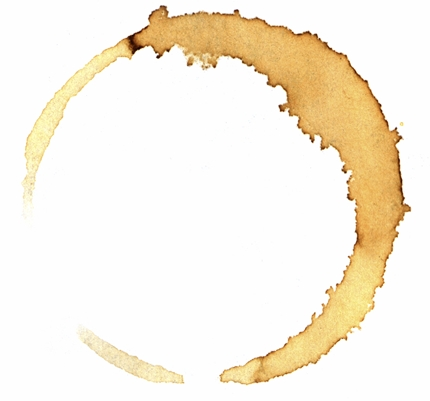
\includegraphics[width=4cm]{./images/cafe-mancha.jpg}
  \end{figure}
  \vspace{-10mm}
  \textbf{\tiny{Apoya tu cafe aqui}} \\
	\vspace{10mm}
  %%%%%%%%%%%%%%%%%%%%%%%%%%%%%%%%%%%%%%
  % Ingresa el mejor titulo que se te ocurra
  %%%%%%%%%%%%%%%%%%%%%%%%%%%%%%%%%%%%%%
	\textbf{\LARGE{Los asistentes de voz, más rápidos, más furiosos!}}\\
	\vspace{4mm}
		\textbf{\large{Tomás Vera\\
  email: \href{mailto:vtomasv@gmail.com}{vtomasv@gmail.com}  } }\\
	\vspace{3mm}
	\textbf{\large{Universidad de Chile}}\\
	\textbf{\small{CC71T-1 Investigación en Cs. de la Computación.(Métodos,Técnicas,Persp.) }}\\
	\textbf{\large{Profesor: Claudio Gutierrez \\
  email: \href{mailto:cgutierr@dcc.uchile.cl}{cgutierr@dcc.uchile.cl}  } }\\
	\today
\end{center}

%%%%%%%%%%%%%%%%%%%%%%%%%%%%%%%%%%%%%%
% Resumen formal de la noticia
%%%%%%%%%%%%%%%%%%%%%%%%%%%%%%%%%%%%%%
\section*{\centering Resumen}
Los desarrolladores de Cortana\autocite{cortana},Google Now\autocite{googleNow} y Siri\autocite{siri} están preocupados, gracias a los avances que el profesor David DeVault a logrado. DeVault y su equipo han desarrollando un sistema de procesamiento del lenguaje de alta velocidad\autocite{entiendo:2016} que aspira a competir en rapidez y eficiencia con el de los hablantes humanos en entornos específicos. Esta es una investigación que cuenta con el apoyo de Universidad del Sur de California\autocite{USC} y la Fundación Nacional de Ciencia\autocite{NSF}, en la actualidad los asistentes por voz tienen una demora en la comprensión y respuesta que sus usuarios realizan, estas demoran rondan entre uno y dos segundos entre que comprenden lo que se les consulta y son capaces de dar respuestas coherentes. Esto estaría por cambiar gracias a DeVault, en su investigación realizaron un juego en el cual le dieron protagonismo a Eve, una agente de procesamiento del lenguaje de alto rendimiento. La dinámica es sencilla: cada jugador ve un conjunto de ocho imágenes en la pantalla de su ordenador. Siempre son las mismas en cada ronda, aunque dispuestas en un orden diferente. A medida que se van resaltando, el jugador debe describirlas mientras el sistema trata de adivinar de qué se trata de la forma más rápida y precisa, para conseguir la puntuación más alta. El experimento permitió mejorar el rendimiento de Eve, con este tipo de entrenamientos se busca optimizar los algoritmos para resolver el reconocimiento de voz, la comprensión del lenguaje y el diálogo. El entrenamiento constante permitió que Eve pudiera responder antes de que el jugador acabara de hablar, permitiendo tener una interacción mucho más natural y fluida, consiguiendo resultados comparables a los obtenidos en el juego entre rivales de carne y hueso.
La aplicación de estos resultados son notables en los campos de los asistentes de voz, también en campos como la automatización de call centers, salud o el entretenimiento, sin embargo 	DeVault subraya "Estamos en el comienzo de un cambio radical en lo que podemos lograr a través de la conversación con los ordenadores", esperemos ver resultados en el corto plazo.


%%%%%%%%%%%%%%%%%%%%%%%%%%%%%%%%%%%%%%
% Tu voz sobre el impacto de esta noticia
%%%%%%%%%%%%%%%%%%%%%%%%%%%%%%%%%%%%%%
\section{Opinion}
El procesamiento de voz\autocite{pvoz}, desde el Reconocimiento de voz hasta reconocimiento de locutores, tiene un potencial muy grande no solo para la ciencia como tal y sus disciplinas sino también para el mercado. Soluciones que permitan identificar en tiempo real a las personas, construir asistentes automáticos para la asistencia de personas de la tercera edad y evidentemente los asistentes de voz de los distintos dispositivos móviles de la actualidad. Adicionalmente recordemos que hoy existe también un mercado bastante desarrollado de otro tipo de asistentes por voz como Echo\autocite{echo} de amazon con Alexa\autocite{alexa}, que pueden verse significativamente favorecidos por este tipo de avances, en sistemas de realización de recetas o como es el caso de Mattel con juguetes\autocite{hbarbie} para niños con una experiencia mucho mas natural.
Con respecto a los avances en Ciencia de la Computación los avances son significativos\autocite{DeVault} tanto en el procesamiento en linea y fuera de linea de voz, también se ven grandes pasos en el desarrollo del entendimiento de lenguaje natural.


%%%%%%%%%%%%%%%%%%%%%%%%%%%%%%%%%%%%%%
% Referencias sobre la noticia
%%%%%%%%%%%%%%%%%%%%%%%%%%%%%%%%%%%%%%
\section{Referencias\label{sec:references}}

\printbibliography[heading=none]


\section{Tu opinion es muy importante!}
\begin{figure}
    \centering
    
\includegraphics[width=4cm]{./images/vote.png}
    \captionsetup{justification=centering, singlelinecheck=false}
\end{figure}

\end{document}
